\chapter{Introducción}

En este \acs{TFG} se desarrolla parte del firmware de un Sistema Empotrado, utilizado para la gestión y control de una motocicleta eléctrica, consistente en el control de un dispositivo GPS y el almacenamiento en un log de los datos recibidos. El componente desarrollado en este documento es parte de un sistema mayor construido por la empresa SmartSoC Solutions. \\

En la actualidad los sistemas empotrados juegan un rol muy importante en muy diversos productos como aplicaciones y servicios en coches, teléfonos móviles, sistemas avanzados de manufactura, equipos médicos, infraestructuras públicas, etc. Los sistemas empotrados suponen un importante aspecto de diferenciación de una empresa dando mejor servicio y experiencia de usuario a sus clientes, representando, en algunos casos, la inversión y desarrollo de este tipo de sistemas hasta el 50\% de su coste operacional \cite{embSistemImport}.\\

Los avances en sistemas empotrados no están limitados únicamente al sector industrial ya que la mayoría de los hitos alcanzados redundan en una mejor calidad de vida de los usuarios o incrementa la productividad y eficiencia de los servicios que realizan. Los sectores que más han implantado sistemas empotrados en su trabajo diario son los relacionados con la sanidad, transporte y logística, seguridad y energía y medio ambiente \cite{embSistemImport}.\\

El tamaño del mercado de los sistemas empotrados es algo difícil de medir ya que son parte de muy diversos productos tecnológicos. Se estima que el volumen de negocio en Holanda en 2014 es de \EUR{73 Millones de} al año y con unas previsiones de crecimiento bastante altas \cite{embSistemImport}.\\
 


\section{Marco de realización del \acs{TFG}}

Este \acs{TFG} se realiza en colaboración con la empresa SmartSoC Solutions y se encuentra enmarcado dentro del proyecto <<BA-2013 Biker Assistant>> de la citada empresa.\\

El proyecto \acs{BA} consiste en la creación de un sistema electrónico completo que gestione y controle los sistemas y comunicaciones de una motocicleta eléctrica. \\

En el desarrollo del proyecto intervienen los siguientes actores:
\begin{itemize}
\item LGN Tech Design, como líder del proyecto. 
\item IS2 del grupo POAS, como coordinador y responsable de electrónica. 
\item Electrónica Viesca, como responsable del sistema de gestión del motor eléctrico. 
\item SmartSoC Solutions, como responsable del firmware del sistema <<Biker Assistant>>. 
\item Grupo ARCO de la UCLM, como desarrollador de firmware.\\
\end{itemize}

El firmware del sistema \acs{BA} ha sido diseñado por SmartSoc Solutions dentro de su ámbito de responsabilidad en el proyecto, siguiendo las especificaciones técnicas y funcionales indicadas por el líder del proyecto.\\

Una vista general del sistema \acs{BA} aparece en la figura \ref{fig:Vision_Sistema_Completo}.\\

El sistema planteado en este \acs{TFG} es el módulo de LOG junto con los sistemas del Sistema de Archivos y las comunicaciones con el dispositivo GPS, como se describe con mayor detalle en el apartado \ref{sec:logGeo}.\\


\begin{figure}[!h]
\begin{center}
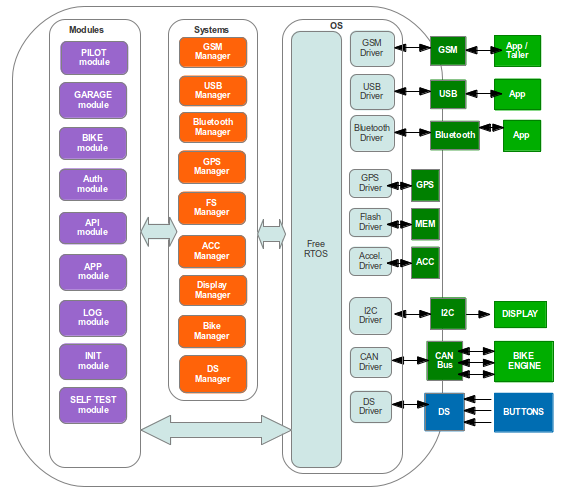
\includegraphics[width=0.68\textwidth]{figs/Vision_Global_Sistema_Completo.png}
\caption{Visión global del sistema <<Biker Assistant>> completo}
\label{fig:Vision_Sistema_Completo}
\end{center}
\end{figure}

\section{Motivación del presente \acs{TFG}}

Dentro del sistema \acs{BA} se debe desarrollar un subsistema de acceso a geolocalización y logging de la misma en tiempo real, que constituye el objetivo de este \acs{TFG}.\\

Este sistema debe ser capaz de recoger información del dispositivo GPS integrado en la placa proporcionada y almacenarlo en su memoria interna.\\

En este \acs{TFG} se explica cómo ha sido diseñado y desarrollado este subsistema, teniendo en cuenta las restricciones de los sistemas empotrados, así como las características de tiempo real necesarias y las específicas del hardware disponible.\\

\section{Subsistema de Logging Geoposicional en Tiempo Real}
\label{sec:logGeo}

El subsistema de Logging Geoposicional en Tiempo Real consta de los siguientes elementos:
\begin{itemize}

\item Acceso al hardware: módulos GPS y memoria Flash.
\item Integración con el sistema operativo en tiempo real.
\item Gestor de alto nivel para el uso del GPS.
\item Sistema de ficheros para la memoria Flash y gestor del mismo.
\item Módulo encargado de realizar el logging del geoposicionamiento.\\

\end{itemize}

En la figura \ref{fig:Vision_Sistema_A_Desarrollar} se puede ver un diagrama general del subsistema.\\
\begin{figure}[!h]
\begin{center}
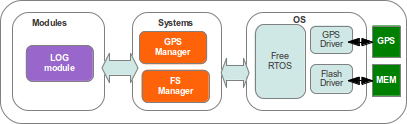
\includegraphics[width=0.5\textwidth]{figs/Vision_Global_Sistema_A_Desarrollar.png}
\caption{Visión global del sistema objetivo de este \acs{TFG}}
\label{fig:Vision_Sistema_A_Desarrollar}
\end{center}
\end{figure}

\section{Retos a afrontar}

Durante la realización del sistema descrito en este \acs{TFG} se deben afrontar varios retos importantes que se describen a continuación.\\

El primer reto afrontado ha sido la configuración del entorno de desarrollo, ya que no existe un entorno oficial y se han tenido que utilizar varias alternativas libres, que cumplen bastante bien su cometido pero que presentan algunos problemas de compatibilidad en determinadas versiones.\\

Otro de los grandes retos afrontados es la utilización de un prototipo hardware diferente al del sistema final, ya que no cuenta con ninguno de los sistemas de interacción con el usuario y la utilización de un un hardware específico que cuenta con sus propias restricciones, como ya se verá más adelante.\\

El reto de desarrollar un sistema en un prototipo hardware que no dispone de ningún componente con el que pueda interactuar el usuario complica notablemente el desarrollo, ya que el sistema se puede probar únicamente a través de la interfaz de programación y depuración.\\

La inestabilidad de los prototipos hardware es otro de los problemas que afrontar. Durante la realización de este \acs{TFG} se produjo un error en uno de los prototipos que provocó la imposibilidad de volver a utilizarlo y se tuvo que remitir a la empresa desarrolladora para que lo revisase.\\

Además, tener un hardware impuesto por la empresa obliga a un estudio más profundo del sistema y la toma de decisiones específicas para completar las funcionalidades requeridas sobre las restricciones inherentes al sistema. Estos problemas se abordan durante el desarrollo del sistema en el Capítulo \ref{chap:desarrollo} fundamentalmente.\\


\section{Estructura del documento}

En el Capítulo \ref{chap:objetivos} se abordan los objetivos del presente \acs{TFG}. Se detalla la división en varias tareas la realización de las funcionalidades planteadas.\\

En el Capítulo \ref{chap:antecedentes} se realiza una visión general sobre los Sistemas Empotrados, los procesos de desarrollo, su historia, el estado actual y su composición. También se habla de la importancia de los Sistemas Operativos en los Sistemas Empotrados y sobre diferentes Sistemas de Archivos.\\

En el Capítulo \ref{chap:desarrollo} se realiza un seguimiento del proceso de desarrollo llevado a cabo, junto con explicaciones detalladas sobre los retos afrontados y las soluciones planteadas.\\

En el Capítulo \ref{chap:resultados} se comparan los resultados obtenidos con los requisitos, tanto funcionales como no funcionales, del sistema propuesto.\\

En el Capítulo \ref{chap:conclusiones} se detallan las conclusiones a las que se han llegado después de realizar este \acs{TFG}.\\

En el Capítulo \ref{chap:trabajoFuturo} se hace un pequeño resumen sobre los mayores problemas afrontados y posibles líneas de trabajo futuro.\\

En el Anexo \ref{anexo:img} se encuentran varias imágenes sobre el hardware utilizado. Además se puede ver sobre una imagen de la placa la localización de sus componentes más característicos.\\

En el Anexo \ref{anexo:coste} se encuentra una estimación de los costes de desarrollo, además del coste final una vez completado el sistema.\\

En el Anexo \ref{anexo:log} se encuentra una pequeña descripción del formato de almacenamiento de los mensajes del GPS en los archivos de log. En este apartado se explica también el motivo por el que se almacena con dicho formato.\\


En el Anexo \ref{anexo:documentacion} se encuentra una completa documentación sobre el sistema desarrollado. Esta documentación ha sido generada por la herramienta Doxygen después de utilizar un formato específico en los comentarios del código fuente.\\
